% Slide 152
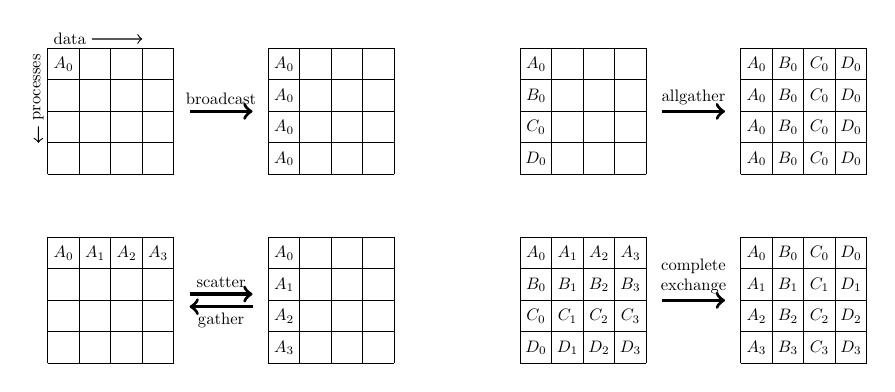
\begin{tikzpicture}[scale = 0.4, every node/.style={scale=0.6}]

\begin{scope}
	\begin{scope}
	\node[anchor = west] (Data) at (0, 4.3) {data};
	\node[anchor = east, rotate = 90] (Proc) at (-0.3, 4) {processes};
	\draw[->] (Data) -- (3, 4.3);
	\draw[->] (Proc) -- (-0.3, 1);
	\draw[step = 1cm] (0,0) grid (4,4);

	\node at (0.5, 3.5) {$A_0$};
	\end{scope}

	\draw[->, very thick] (4.5, 2) -- node[midway, above] {broadcast} (6.5, 2);

	\begin{scope}[xshift = 7cm]
	\draw[step = 1cm] (0,0) grid (4,4);

	\foreach \y in {0.5, 1.5, ..., 3.5}
		\node at (0.5, 4 - \y) {$A_0$};
	\end{scope}

	\begin{scope}[yshift = -6cm]
	\draw[step = 1cm] (0,0) grid (4,4);

	\foreach \x [count = \i from 0] in {0.5, 1.5, ..., 3.5}
		\node at (\x, 3.5) {$A_\i$};
	\end{scope}

	\draw[->, very thick] (4.5, -3.8) -- node[midway, above] {scatter} (6.5, -3.8);
	\draw[<-, very thick] (4.5, -4.2) -- node[midway, below] {gather} (6.5, -4.2);

	\begin{scope}[yshift = -6cm, xshift = 7cm]
	\draw[step = 1cm] (0,0) grid (4,4);

	\foreach \x [count = \i from 0] in {0.5, 1.5, ..., 3.5}
		\node at (0.5, 4 - \x) {$A_\i$};
	\end{scope}
\end{scope}

\begin{scope}[xshift = 15cm]
	\begin{scope}[yshift = 0cm]
	\draw[step = 1cm] (0,0) grid (4,4);

	\foreach \y/\l in {0.5/A, 1.5/B, 2.5/C, 3.5/D}
		\node at (0.5, 4 - \y) {$\l_0$};
	\end{scope}

	\draw[->, very thick] (4.5, 2) -- node[midway, above] {allgather} (6.5, 2);

	\begin{scope}[yshift = 0cm, xshift = 7cm]
	\draw[step = 1cm] (0,0) grid (4,4);

	\foreach \y in {0.5, 1.5, ..., 3.5} {
		\foreach \x/\l in {0.5/A, 1.5/B, 2.5/C, 3.5/D} {
			\node at (\x, 4 - \y) {$\l_0$};
		}
	}
	\end{scope}

	\begin{scope}[yshift = -6cm]
	\draw[step = 1cm] (0,0) grid (4,4);

	\foreach \y/\l in {0.5/A, 1.5/B, 2.5/C, 3.5/D} {
		\foreach \x[count = \i from 0] in {0.5, 1.5, ..., 3.5} {
			\node at (\x, 4 - \y) {$\l_\i$};
		}
	}
	\end{scope}

	\draw[->, very thick] (4.5, -4) -- node[midway, above, align = center] {complete \\ exchange} (6.5, -4);

	\begin{scope}[yshift = -6cm, xshift = 7cm]
	\draw[step = 1cm] (0,0) grid (4,4);

	\foreach \x/\l in {0.5/A, 1.5/B, 2.5/C, 3.5/D} {
		\foreach \y[count = \i from 0] in {0.5, 1.5, ..., 3.5} {
			\node at (\x, 4 - \y) {$\l_\i$};
		}
	}
	\end{scope}
\end{scope}

\end{tikzpicture}
